\chapter{The Nature of Numbers}\label{chapter:induction}

\section{On the Concept of Number Throughout History}

Many people are familiar with numbers through everyday experiences like counting, measuring, or comparing quantities. From a young age, we develop an intuition about how numbers behave. Our experience with numbers reveals patterns of truths and properties that seem to always be true. For example, we quickly learn that it does not matter in which order we add two numbers: Given two numbers $a$ and $b$ it is always true that $a+b=b+a$. Truths such as this one seem so self-evident that we might be tempted to just accept them. However, for a rigorous mathematical theory we need to be more careful. Mathematicians require proofs—conclusive arguments that establish why certain properties hold universally for all numbers, or at least for precisely defined sets of numbers. Checking a property for every number up to a hundred, a million, or even $10^{27}$ might confirm a pattern, but infinitely many numbers remain beyond such finite checks. To reason about all natural numbers at once, we need formal principles that extend beyond empirical observation and anecdotal evidence. In order to discover such reasoning principles, we need to find out what the natural numbers really are.

Although natural numbers arise from counting, the notion of number is not inherently linked to any particular collection of entities being counted. Scholars in the Pythagorean tradition were among the first to articulate this insight. Nicomachus emphasized the concepts of \emph{monad}, \emph{dyad}, and \emph{triad} for the totality of all things that come in one, two, or three units \cite{nicomachus1926}. Nicomachus ascribed divine properties to the monad, or unity: ``{\it It generates itself without beginning, without end, and appears to be the cause of enduring, as God in the realm of physical actualities is in such manner perceived of as a preserving and guarding agent of nature}''. Nicomachus drew strong parallels between the monad and the concept of sameness, and likewise between the dyad and the concept of otherness. He also emphasized that numbers were composed of monads. In other words, the monad is the source of all numbers. Although mathematicians do not ascribe divine properties to numbers anymore, we see here the emergence of some important ideas. The first is that all numbers are generated from the monad, that is, unity. The second idea is to connect unity with sameness. The idea that all things equal to a given object form a unit, or a singleton, anticipates a fundamental principle of equality. However, we shall forego the interesting digressions that we could make about equality and focus our attention on the concept of number.

With Euclid, we see a shift away from the divine conception of the monad. For Euclid, a \emph{unit} is the conceptual principle by which an individual object is identified as one, and a \emph{number} is a multitude composed of such units in a discrete fashion \cite{euclid2015}. In other words, the concept of unit captures the notion of oneness, but this is distinct of the number $1$ itself. Both Nicomachus's and Euclid's views on the concept of number were highly influential throughout late antiquity and the Middle Ages, particularly through Boethius's Latin rendition of Nicomachus's \emph{Introduction to Arithmetic} and Adelard of Bath's translation of Euclid's \emph{Elements}.

While Pierre de Fermat is regarded the founder of modern number theory, he did not write extensively on the philosophy of mathematics. Nevertheless, certain themes in his correspondence and work show a clear orientation. For him, mathematics is about truths intrinsic to numbers. Numbers were the object of exact reasoning. He emphasized that \emph{induction}, by which mathematicians up to the early 19th century understood experimental verification, was insufficient to establish universal truths of numbers. Among Fermat’s lasting contributions was his method of infinite descent, a method of proof by contradiction in which one shows that any supposed solution would lead to an ever-decreasing sequence of natural numbers, which is impossible.

With Euler, we witness a significant conceptual expansion. In his \emph{Elements of Algebra}, Euler extended the notion of number beyond the natural and rational to encompass negative numbers, irrationals, complex numbers, and even infinite series. He was among the first to conjecture that constants like $e$ and $\pi$ are transcendental; that is, not the roots of any algebraic equation with rational coefficients. For Euler, numbers were entities governed by formal laws, irrespective of whether they corresponded to geometric magnitudes. Euler's broadening of the concept of numbers, and his use of analytic methods would eventually spark debates about the foundations of mathematics and the logical principles underlying mathematical truth.

In the 19th century, the nature of mathematics itself began to change. The emergence of non-Euclidean geometry was a challenge to the status of Euclid's Elements as the de facto foundation of mathematics. Weierstrass's discovery of continuous, nowhere differentiable functions underscored the need for a more solid foundation of calculus, and with Galois's use of symmetries in order to show that quintic equations had no solutions expressible in terms of radicals abstract algebra started to become more prominent.

We view the set of numbers as an abstract entity that exist as a precisely specified concept within the collective imagination of conscious beings to convey and communicate ideas such as counting, comparing, and measuring quantities.

When we say that the natural numbers are the numbers $0$, $1$, $2$, $\ldots$, we really mean that the natural numbers are generated from $0$ and the \define{successor function} $n\mapsto n+1$. The collection of all natural numbers forms a set or type

\begin{equation}
  \mathbb{N}:=\{0,1,2,\ldots\}.
\end{equation}

Mathematicians often prefer to work with sets, while computer scientists might prefer to work with types, both of which are collections of abstract objects often referred to as \define{elements}. The distinction is merely that of the logical framework being used: Most mathematicians rely on the Zermelo--Fraenkel set theory, while computer scientist rely on programming languages that often have a type theory in its foundation. Theorem proving in computer programs called \emph{proof assistants} is rapidly becoming a more essential mathematical activity for students and researchers alike. However, many of the most popular proof assistants are based on type theory, in which collections of mathematical objects are called types.

\section{Induction and Recursion}

The natural number zero and the successor function together are sufficient to describe all the natural numbers. The mathematician's way to express this sufficiency is by stating the principle of \define{mathematical induction}: Given any property $P(n)$ expressing a condition of an arbitrary natural number $n$, in order to prove that $P(n)$ is true for all $n$ it suffices to prove that:
\begin{enumerate}
\item The property $P(0)$ is true.
\item For all $n$, if the property $P(n)$ holds then the property $P(n+1)$ holds.
\end{enumerate}
Mathematical induction works, because every natural number is either $0$ or it is the successor of a previous natural number. Proving a property for all natural numbers therefore breaks down in two cases: The \define{base case} in which we prove that $P(0)$ is true, and the \define{inductive step} where we prove that $P(n+1)$ is true provided that $P(n)$ is true.

Proofs by induction can be broken down into the following steps: First identify the property $P(n)$ that you want to prove by induction. The goal of an induction proof is to prove that $P(n)$ is true for all $n$. Then prove the base case. While this step is often trivial, it is a necessary and essential part of an induction proof. Finally, for the inductive step, write down the exact induction hypothesis, namely the property $P(n)$, and the exact goal of the inductive step, namely the property $P(n+1)$. Then use the induction hypothesis to prove that $P(n+1)$ then also holds. After these steps the proof that $P(n)$ holds is complete.

Since we have previously defined the set of natural numbers to be a set equipped with an element $0$ and a function $S$, satisfying an induction principle, it is of some importance to demonstrate that this definition is sufficiently strong to define familiar operations on the natural numbers, such as addition and multiplication, and to verify their laws.

This naturally leads us to the principle of \define{recursion}, which allows us to define certain operation by a mechanism that is not unlike induction. While the induction principle of the natural numbers is used to \emph{prove} properties uniformly about the natural numbers, recursion is a way to \emph{define} functions, operations, and sequences of elements. Its general principle is that if we wish to specify a function $f:\mathbb{N}\to X$ by recursion, then we have to specify its value at $0$ and its value at $n+1$ using an expression that possibly refers to $n$ and the value $f(n)$. More precisely, a function $f$ is defined by recursion as follows:
\begin{align*}
  f(0) & := x_0 \\
  f(n+1) & := h(n,f(n)).
\end{align*}
Here $h$ is a function that is previously defined. If we define $f$ in this way, then by definition $f$ satisfies the equalities
\begin{align*}
  f(0) & = x_0 \\
  f(n+1) & = h(n,f(n)).
\end{align*}

An important special case of recursion, by which we will define many examples of recursive functions, is to iterate any function $f$ on any set $X$: We define the $n$th iteration $f^n$ of $f$ by
\begin{align*}
  f^0(x) & := x \\
  f^{n+1}(x) & := f(f^n(x)). 
\end{align*}
In other words, the $0$th iteration of $f$ is the \define{identity function}, which leaves all elements untouched, and the $(n+1)$st iteration of $f$ is obtained by applying $f$ once more to the values of the $n$th iteration of $f$.

Notice that we made a choice in the definition of the $(n+1)$st iteration of $f$. We could have defined it alternatively by $f^{n+1}(x):=f^n(f(x))$. In the following proposition we will prove by induction that this leads to the same definition.

\begin{proposition}\label{proposition:iterate-successor}
  Consider a function $f:X\to X$ on a set $X$, and let $n$ be a natural number. Then we have
  \begin{equation*}
    f^{n+1}(x) = f^n(f(x))
  \end{equation*}
  for all $x\in X$.
\end{proposition}

\begin{proof}
  The proof is by induction on $n$. In the base case, we must show that
  \begin{equation*}
    f^1(x) = f^0(f(x)).
  \end{equation*}
  By our definition of $f^n(x)$, we have that $f^1(x)=f(f^0(x))$, and we have $f^0(x)=x$, so that
  \begin{equation*}
    f^1(x)=f(f^0(x))=f(x)=f^0(f(x)).
  \end{equation*}
  This proves the base case. In the inductive step, we assume as our inductive hypothesis that
  \begin{equation*}
    f^{n+1}(x)=f^n(f(x))
  \end{equation*}
  for every $x\in X$. Our goal is then to show that
  \begin{equation*}
    f^{n+2}(x)=f^{n+1}(f(x)).
  \end{equation*}
  Here we use that $f^{n+1}(y)=f(f^n(y))$ for all $y\in X$. Indeed, this allows us to complete the proof:
  \begin{equation*}
    f^{n+2}(x) = f(f^{n+1}(x)) = f(f^n(f(x)))=f^{n+1}(f(x)).\qedhere
  \end{equation*}
\end{proof}

\section{Addition of Natural Numbers}

\begin{definition}
  The \define{addition operation} ${+}:\mathbb{N}\to\mathbb{N}\to\mathbb{N}$ is a binary operation defined by iterating the successor function $S$:
  \begin{equation*}
    m+n := S^n(m).
  \end{equation*}
  In other words, $m+n$ is the $n$th successor of $m$.
\end{definition}

The operation $m,n\mapsto m+n$ satisfies the equalities
\begin{align*}
  m+0 & = m \\
  m+(n+1) & = (m+n)+1
\end{align*}
by definition. However, the equalities
\begin{align*}
  0+n & = n \\
  (m+1)+n & = (m+n)+1
\end{align*}
require a short proof.

\begin{proposition}\label{proposition:unit-law-addition-nat}
  For any two natural numbers $m$ and $n$ we have
  \begin{align*}
    0+n & = n \\
    (m+1)+n & = (m+n)+1.
  \end{align*}
\end{proposition}

\begin{proof}
  The proof of both equalities is by induction on $n$. For the base case of the first equality, note that the equality $0+0=0$ holds by definition. For the inductive step, assume that $0+n=n$. Then we have
  \begin{equation*}
    0+(n+1)=(0+n)+1= n+1.
  \end{equation*}
  For the base case of the second equality, note that the equalities $(m+1)+0=m+1=(m+0)+1$ hold by definition. For the inductive step, assume that $(m+1)+n=(m+n)+1$. Then we have
  \begin{equation*}
    (m+1)+(n+1)=((m+1)+n)+1=((m+n)+1)+1=(m+(n+1))+1.\qedhere
  \end{equation*}
\end{proof}

\begin{proposition}\label{proposition:iterate-add}
  For any function $f:X\to X$, we have
  \begin{equation*}
    f^{m+n}(x)=f^m(f^n(x)).
  \end{equation*}
\end{proposition}

\begin{proof}
  The proof is by induction on $n$. In the base case, we have $m+0=m$ and $f^0(x)=x$. Together, these identities give:
  \begin{equation*}
    f^{m+0}(x)=f^m(x)=f^m(f^0(x)).
  \end{equation*}
  For the inductive step, assume that for every element $x\in X$ we have $f^{m+n}(x)=f^m(f^n(x))$. Our goal is to show that
  \begin{equation*}
    f^{m+(n+1)}(x)=f^m(f^{n+1}(x)).
  \end{equation*}
  Here, we use that $m+(n+1)=(m+n)+1$ and that $f^{n+1}(x)=f(f^n(x))$ hold by definition, and that $f^m(f(x))=f(f^m(x))$ by \cref{proposition:iterate-successor}. Together, these identities give:
  \begin{equation*}
    \begin{split}
      f^{m+(n+1)}(x)=f^{(m+n)+1}(x) & =f(f^{m+n}(x))=f(f^m(f^n(x))) \\
                                    & =f^m(f(f^n(x)))=f^m(f^{n+1}(x)).\qedhere
    \end{split}
  \end{equation*}
\end{proof}

\begin{corollary}
  Addition of natural numbers is \define{associative}: For any three natural numbers $l$, $m$, and $n$ we have
  \begin{equation*}
    (l+m)+n = l+(m+n).
  \end{equation*}
\end{corollary}

\begin{proof}
  By definition, we have $(l+m)+n=S^n(S^m(l))$ and $l+(m+n)=S^{m+n}(l)$. Combining these identities with \cref{proposition:iterate-add}, we obtain
  \begin{equation*}
    (l+m)+n=S^n(S^m(l))=S^{m+n}(l)=l+(m+n).\qedhere
  \end{equation*}
\end{proof}

\begin{proposition}
  Addition of natural numbers is \define{commutative}: For any two natural numbers $m$ and $n$, we have
  \begin{equation*}
    m+n=n+m.
  \end{equation*}
\end{proposition}

\begin{proof}
  The proof is by induction on $n$. In the base case, we use \cref{proposition:unit-law-addition-nat}
  \begin{equation*}
    m+0=m=0+m.
  \end{equation*}
  For the inductive step, assume that $m+n=n+m$. Then we use \cref{proposition:unit-law-addition-nat} again to obtain:
  \begin{align*}
    m+(n+1) & = (m+n)+1 \\
            & = (n+m)+1 \\
            & = (n+1)+m.\qedhere
  \end{align*}
\end{proof}

Some further useful identifications of addition, which follow from the associativity and commutativity laws, are:
\begin{align*}
  (l+m)+n & = (l+n)+m \\
  l+(m+n) & = m+(l+n) \\
  (k+l)+(m+n) & = (k+m)+(l+n).
\end{align*}
The last identification is called the \define{interchange law} for addition. The first one follows from the second, and the second and third are proven by a short calculation:
\begin{align*}
  l+(m+n) & = (l+m)+n & (k+l)+(m+n) & = k+(l+(m+n)) \\
          & = (m+l)+n & & = k + (m + (l+n)) \\
          & = m+(l+n) & & = (k+m)+(l+n).
\end{align*}

\section{Arithmetic of Natural Numbers}

\begin{definition}
  The multiplication function $m,n\mapsto mn$ on the natural numbers is defined recursively by
  \begin{align*}
    m0 & := 0 \\
    m(n+1) & := mn + m.
  \end{align*}
\end{definition}

\begin{proposition}
  Multiplication of natural numbers satisfies the following laws:
  \begin{align*}
    0n & = 0 & m0 & = 0 \\
    (m+1)n & = mn+n & m(n+1) & = mn+m \\
    1m & = m & m1 & = m \\
    l(m+n) & = lm+ln & (l+m)n & = ln+mn \\
    (lm)n & = l(mn) & mn & = nm.
  \end{align*}
\end{proposition}

\begin{proof}
  We prove that $0n=0$ by induction on $n$. In the base case, we have the equality $00=0$. For the inductive step, assume that $0n=0$. Then $0(n+1)=0n+0=0n=0$, completing the proof of the first identity. The identity $m0=0$ holds by definition.

  The proof that $(m+1)n=mn+n$ is again by induction on $n$. In the base case, we have the equalities $(m+1)0=0=m0=m0+0$. For the inductive step, assume that $(m+1)n=mn+n$. Then we have
  \begin{equation*}
    (m+1)(n+1)=(m+1)n+(m+1)=(mn+n)+(m+1)=(mn+m)+(n+1)=m(n+1)+(n+1).
  \end{equation*}
  The identity $m(n+1)=mn+m$ holds by definition.

  Next, we prove first that $mn=nm$, by induction on $n$. In the base case, we have the equalities $m0=0=0m$. For the inductive step, assume that $mn=nm$. Then we have that
  \begin{equation*}
    m(n+1)=mn+m=nm+m=(n+1)m.
  \end{equation*}

  Now we prove that $l(m+n)=lm+ln$. We prove it by induction on $n$. In the base case, we have that $l(m+0)=lm=lm+0= lm+l0$. For the inductive step, assume that $l(m+n)=lm+ln$. Then we have that
  \begin{equation*}
    l(m+(n+1))=l((m+n)+1)=l(m+n)+l=(lm+ln)+l=lm+(ln+l)=lm+l(n+1).
  \end{equation*}
  The identification $(l+m)n=ln+mn$ follows from the previous identification, using the fact that $mn=nm$.

  Finally, the proof that $(lm)n=l(mn)$ is by induction on $n$. In the base case, we have the equalities $(lm)0=0=l0=l(m0)$. For the inductive step, assume that $(lm)n=l(mn)$. Then we have that
  \begin{equation*}
    (lm)(n+1)= (lm)n+lm=l(mn)+lm=l(mn+m)=l(m(n+1)).
  \end{equation*}
\end{proof}

\section{Finite Sums and Products}

\begin{definition}
  The \define{finite summation operation} $\sum$ is defined by specifying a finite subset $I\subseteq \mathbb{N}$ and a family of natural numbers $a_i$ where $i$ ranges over the elements of $I$. We will write
  \begin{equation*}
    \sum_{i\in I}a_i
  \end{equation*}
  for the sum over all the natural numbers $a_i$, with $i$ ranging over $I$. This sum is defined by recursion over the number of elements in $I$. If $I$ has no elements (that is, $I$ is empty), then we define
  \begin{equation*}
    \sum_{i\in I}a_i := 0.
  \end{equation*}
  If $I$ has at least one element $i_0$, then we write $J:=I\setminus\{i_0\}$, allowing us to define
  \begin{equation*}
    \sum_{i\in I}a_i := a_{i_0}+\sum_{i\in J}a_j.
  \end{equation*}
\end{definition}

\begin{theorem}
  For any natural number $n$ we have
  \begin{equation*}
    0 + \cdots + n = \frac{n(n+1)}{2}.
  \end{equation*}
\end{theorem}

\begin{proof}
  Let $S_n:=0+\cdots+n$, and let $P(n)$ be the property that $S_n=\frac{n(n+1)}{2}$. We will prove that $P(n)$ is true for all $n$ by induction. In the base case, we have to show that $P(0)$ holds, that is, that the identity
  \begin{equation*}
    0=\frac{0\cdot 1}{2}
  \end{equation*}
  is true. This is indeed true, because the numerator in the fraction on the right-hand side is $0$.

  For the induction step, let $n$ be a natural number and assume as our inductive hypothesis that $P(n)$ is true. Our goal is now to prove $P(n+1)$, that is, that the identity
  \begin{equation*}
    S_{n+1}=\frac{(n+1)(n+2)}{2}.
  \end{equation*}
  Note that $S_{n+1}=S_n+(n+1)$. By the inductive hypothesis we have that $S_n=\frac{n(n+1)}{2}$, which we may now use to rewrite
  \begin{equation*}
    S_n + (n+1) = \frac{n(n+1)}{2} + (n+1).
  \end{equation*}
  Observe that $(n+1)=\frac{2(n+1)}{2}$. Therefore we can make the following computation:
  \begin{equation*}
    \frac{n(n+1)}{2} + (n+1) = \frac{n(n+1)}{2}+\frac{2(n+1)}{2} = \frac{n(n+1)+2(n+1)}{2}=\frac{(n+2)(n+1)}{2}.
  \end{equation*}
  Since $(n+2)(n+1)=(n+1)(n+2)$ it follows that $S_{n+1}=\frac{(n+1)(n+2)}{2}$ as desired.
\end{proof}

We illustrate induction with another example, the \define{formula for the geometric series}.

\begin{theorem}\label{theorem:formula-geometric-series}
  For any real number $x$ not equal to $1$, the identity
  \begin{equation*}
    \sum_{k=0}^{n-1}x^k = \frac{x^n-1}{x-1}.
  \end{equation*}
\end{theorem}

\begin{proof}
  The proof is by induction on $n$. In the case $n=0$ the sum
  \begin{equation*}
    \sum_{k=0}^{-1}x^k
  \end{equation*}
  is an empty sum, because it sums over all elements $0\leq k \leq -1$ of which there are none. In empty sums, nothing is being added, so they are always $0$. On the right hand side, we also see that
  \begin{equation*}
    \frac{x^0-1}{x-1}=\frac{1-1}{x-1}=0,
  \end{equation*}
  and hence the base case holds.

  For the inductive step, assume that $\sum_{k=0}^{n-1}x^k=\frac{x^n-1}{x-1}$. Our goal is to show that
  \begin{equation*}
    \sum_{k=0}^{n}x^k=\frac{x^{n+1}-1}{x-1}.
  \end{equation*}
  Note that $\sum_{k=0}^{n}x^k=(\sum_{k=0}^{n-1}x^k)+x^n$. By applying the induction hypothesis we therefore find that
  \begin{equation*}
    \sum_{k=0}^{n}x^k=\frac{x^n-1}{x-1}+x^n.
  \end{equation*}
  Note that $x^n=\frac{(x-1)x^n}{x-1}$. Therefore we can bring the two summands under one fraction as follows:
  \begin{equation*}
    \frac{x^n-1}{x-1}+x^n=\frac{x^n-1}{x-1}+\frac{(x-1)x^n}{x-1}=\frac{x^n-1+x^{n+1}-x^n}{x-1}=\frac{x^{n+1}-1}{x-1}.
  \end{equation*}
  This completes the inductive step, and therefore the proof.
\end{proof}

\section{A First Counting Problem}

\begin{figure}[b]
  \centering
  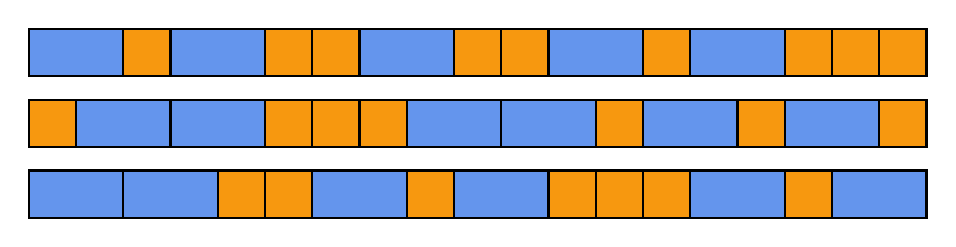
\begin{tikzpicture}[scale=0.6]
    % --- first tiling (a) at y=0 ---
    \begin{scope}[shift={(0,0)}]
      % tiles: 2,1,2,1,1,2,1,1,2,1,2,1,1,1
      \foreach \x/\len in {
        0/2, 2/1, 3/2, 5/1, 6/1, 7/2, 9/1,
        10/1, 11/2, 13/1, 14/2, 16/1, 17/1, 18/1
      }{
        \ifnum\len=1
          \fill[YellowOrange] (\x,0) rectangle ++(1,1);
        \else
          \fill[CornflowerBlue] (\x,0) rectangle ++(2,1);
        \fi
        \draw[thick] (\x,0) rectangle ++(\len,1);
      }
    \end{scope}
    
    % --- second tiling (b) at y=-1.5 ---
    \begin{scope}[shift={(0,-1.5)}]
      % tiles: 1,2,2,1,1,1,2,2,1,2,1,2,1
      \foreach \x/\len in {
        0/1, 1/2, 3/2, 5/1, 6/1, 7/1, 8/2,
        10/2, 12/1, 13/2, 15/1, 16/2, 18/1
      }{
        \ifnum\len=1
          \fill[YellowOrange] (\x,0) rectangle ++(1,1);
        \else
          \fill[CornflowerBlue] (\x,0) rectangle ++(2,1);
        \fi
        \draw[thick] (\x,0) rectangle ++(\len,1);
      }
    \end{scope}
    
    % --- third tiling (c) at y=-3 ---
    \begin{scope}[shift={(0,-3)}]
      % tiles: 2,2,1,1,2,1,2,1,1,1,2,1,2
      \foreach \x/\len in {
        0/2, 2/2, 4/1, 5/1, 6/2, 8/1, 9/2,
        11/1, 12/1, 13/1, 14/2, 16/1, 17/2
      }{
        \ifnum\len=1
          \fill[YellowOrange] (\x,0) rectangle ++(1,1);
        \else
          \fill[CornflowerBlue] (\x,0) rectangle ++(2,1);
        \fi
        \draw[thick] (\x,0) rectangle ++(\len,1);
      }
    \end{scope}
  \end{tikzpicture}
  \caption[Some Fibonacci tilings of a 1-by-19 grid]{\label{figure:fibonacci-tilings}Three example tilings of a 1-by-19 grid using monominoes (1-by-1 tiles) and dominoes (1-by-2 tiles).}
\end{figure}

Consider the set of patterns one can make on a 1-by-$n$ grid using monominoes (1-by-1 tiles) and dominoes (1-by-2 tiles). In \cref{figure:fibonacci-tilings} we have displayed some examples. How many such patterns are there?

In order to count them, let $T(n)$ be the number of such tilings. One way of finding the number $T(n)$, which works when a specific $n$ is given, is to simply list all the tilings of a 1-by-$n$ grid. Doing so for small values of $n$ is a great way to get a feeling for the problem. In \cref{figure:complete-fifth-fibonacci-tiling} we have listed all the possible tilings of the 1-by-5 grid.
\begin{figure}[t]
  \centering
  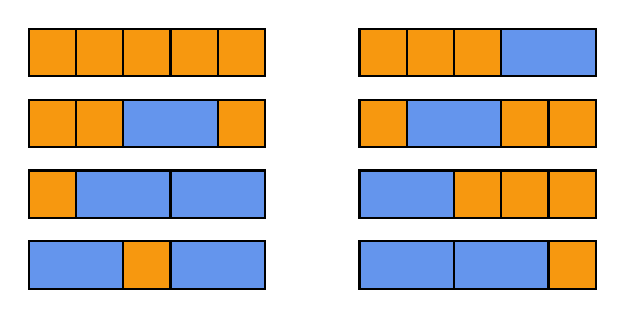
\begin{tikzpicture}[scale=0.6]
    % Colours
    \definecolor{mono}{RGB}{255,165,0}   % monomino
    \definecolor{domi}{RGB}{100,149,237} % domino
    
    % Helper: draw one tiling given a shift and a list of x/length pairs
    \newcommand{\drawtiling}[3]{%
      \begin{scope}[shift={(#1,#2)}]
        \draw[step=1cm,gray!40] (0,0) grid (5,1);
        \foreach \x/\len in {#3} {
          \ifnum\len=1
            \fill[YellowOrange] (\x,0) rectangle ++(1,1);
            \draw[thick] (\x,0) rectangle ++(1,1);
          \else
            \fill[CornflowerBlue] (\x,0) rectangle ++(2,1);
            \draw[thick] (\x,0) rectangle ++(2,1);
          \fi
        }
      \end{scope}%
    }
    
    % Now place the 8 tilings in two columns
    % Each list is x/length so that the tiles exactly fill 0..5
    \drawtiling{0}{   0}{0/1,1/1,2/1,3/1,4/1}   % 1 1 1 1 1
    \drawtiling{7}{   0}{0/1,1/1,2/1,3/2}       % 1 1 1 2
    \drawtiling{0}{ -1.5}{0/1,1/1,2/2,4/1}      % 1 1 2 1
    \drawtiling{7}{ -1.5}{0/1,1/2,3/1,4/1}      % 1 2 1 1
    \drawtiling{7}{ -3  }{0/2,2/1,3/1,4/1}      % 2 1 1 1
    \drawtiling{0}{ -3  }{0/1,1/2,3/2}          % 1 2 2
    \drawtiling{0}{ -4.5}{0/2,2/1,3/2}          % 2 1 2
    \drawtiling{7}{ -4.5}{0/2,2/2,4/1}          % 2 2 1
    
  \end{tikzpicture}  
  \caption[Fibonacci tilings of a 1-by-5 grid]{\label{figure:complete-fifth-fibonacci-tiling}A list of all the possible tilings of a 1-by-5 grid using monominoes and dominoes.}
\end{figure}

However, listing all such tilings gets elaborate quite quickly, and furthermore doing so by hand is quite error-prone. The problem is therefore to find a clever way of counting all possible patterns for all $n$.

Notice that the last tile is either a monomino or a domino, so there are two cases to consider. The number of tilings ending in a monomino is exactly the number $T(n-1)$, and the number of tilings ending in a domino is exactly the number $T(n-2)$. Thus, the total number of tilings of a 1-by-$n$ grid is the sum of these two numbers:
\begin{equation*}
  T(n) = T(n-1)+T(n-2).
\end{equation*}
This is exactly the same recursive rule as for the Fibonacci numbers!

To complete the computation of $T(n)$, we have to determine how the sequence $T(n)$ starts off. That is, we need to determine $T(1)$ and $T(2)$. There is exactly one way to tile a 1-by-1 grid using monominoes and dominoes, namely by using one monomino, and there are two ways of tiling a 1-by-2 grid using monominoes and dominoes, namely by using either two monominoes or one domino. We therefore find that $T(1)=1$ and $T(2)=2$, and we can therefore conclude that
\begin{equation*}
  T(n) = F_{n+1}.
\end{equation*}
This tiling interpretation of the Fibonacci numbers appears in \cite{brigham1996}, though equivalent counting problems have a much older origin. In the 12th century, the Indian scholars Gopāla and Hemachandra studied the number of rhythmic patterns formed by combining short and long syllables in Sanskrit prosody. Hemachandra, around the year 1150, gave a precise formulation of the recurrence relation now associated with the Fibonacci sequence, and listed the initial values: $1$, $2$, $3$, $5$, $8$, $13$, $21$. His results appear in his treatise on metrics, the \emph{Chandonuśāsana} \cite{hemachandra1961}, composed several decades before Fibonacci’s \emph{Liber Abaci} (1202). These numbers are therefore sometimes referred to as the \emph{Hemachandra numbers}.

The delightful book \emph{Proofs That Really Count: The Art of Combinatorial Proof} by Arthur Benjamin and Jennifer Quinn uses the tiling interpretation of the Fibonacci numbers to derive many Fibonacci identities combinatorially, and it contains many further examples of beautiful counting constructions \cite{benjamin2003}.

\begin{exercises}
  \exercise \label{exercise:difference-of-powers}Prove the \define{formula for the difference of $n$th powers}
  \begin{equation*}
    x^n-y^n=(x-y)\sum_{k=0}^{n-1}x^ky^{n-1-k}.
  \end{equation*}
  Note that this formula generalizes the \define{formula for the difference of squares}
  \begin{equation*}
    x^2-y^2 = (x-y)(x+y)
  \end{equation*}
  as well as the formula for the geometric series
  \begin{equation*}
    x^n-1=(x-1)\sum_{k=0}^{n-1}x^k.
  \end{equation*}
  % \exercise \emph{Sophie Germain's identity.} Show that
  % \begin{equation*}
  %   a^4+4b^4=(a^2-2ab+2b^2)(a^2+2ab+2b^2).
  % \end{equation*}
  \exercise \label{exercise:identities-triangular-numbers}Write $T_n$ for the $n$th triangular number.
  \begin{subexenum}
  \item For $0\leq m<n$, show that
    \begin{equation*}
      T_n-T_m=\frac{(n-m)(n+m+1)}{2}.
    \end{equation*}
  \item For any two natural numbers $m$ and $n$, show that
    \begin{equation*}
      T_{m+n}=T_{m}+T_n+mn.
    \end{equation*}
  \item Show that
    \begin{equation*}
      T_{2n}=4T_n-n.
    \end{equation*}
  % \item Show that
  %   \begin{equation*}
  %     T_{2n}=2T_n+n^2.
  %   \end{equation*}
  % \item Show that
  %   \begin{equation*}
  %     T_{kn}=k^2T_n-nT_{k-1}.
  %   \end{equation*}
  \item Show that
    \begin{equation*}
      8T_n+1=(2n+1)^2.
    \end{equation*}
  \end{subexenum}
  \exercise \label{exercise:sum-of-odd-numbers}Prove that that the sum of the first $n$ odd numbers is a perfect square. That is, prove that
  \begin{equation*}
    \sum_{k=0}^{n-1} 2k+1 = n^2.
  \end{equation*}
  Note: This summation formula is the starting point from which Fibonacci derived much of his work in his book  \emph{Liber Quadratorum (The Book of Squares)} \cite{fibonacci1987}.
  \exercise Write $T_n$ for the $n$th triangular number.
  \begin{subexenum}
  \item The numbers
    \begin{equation*}
      S_n:=\sum_{k=0}^nT_k
    \end{equation*}
    are called the \emph{tetrahedral numbers}. Give a geometric interpretation of these numbers justifying their name.
  \item Prove that
    \begin{equation*}
      S_n = \frac{n(n+1)(n+2)}{6}.
    \end{equation*}
  \item Prove that
    \begin{equation*}
      S_{m+n}=S_m+S_n+\frac{mn(m+n+2)}{2}.
    \end{equation*}
  \end{subexenum}
  \exercise Prove the \define{formula for the square pyramidal numbers}
  \begin{equation*}
    \sum_{k=0}^n k^2 = \frac{n(n+1)(2n+1)}{6}.
  \end{equation*}
  Can you explain why the numbers of the form $\sum_{k=0}^n k^2$ are called square pyramidal numbers?
  \exercise Prove that
  \begin{equation*}
    \sum_{k=0}^{n-1}(2k+1)^2 = \frac{n(4n^2-1)}{3}.
  \end{equation*}
  \exercise Prove \define{Nicomachus's Theorem}
  \begin{equation*}
    \sum_{k=0}^n k^3 = \left(\sum_{k=0}^{n}k\right)^2.
  \end{equation*}
  \exercise Prove that
  \begin{equation*}
    \sum_{k=0}^{n-1}(2k+1)^3=n^2(2n^2-1).
  \end{equation*}
  \exercise Prove that
  \begin{equation*}
    \sum_{k=0}^n k(k+1)(k+2) = \frac{n(n+1)(n+2)(n+3)}{4}.
  \end{equation*}
  \exercise Consider the Fibonacci numbers $F(n)$ given by
  \begin{align*}
    F_0 & := 0 \\
    F_1 & := 1 \\
    F_{n+2} & := F_{n+1}+F_n.
  \end{align*}
  Prove that
  \begin{equation*}
    \sum_{k=0}^nF_k = F_{n+2}-1.
  \end{equation*}
  \exercise Prove that
  \begin{equation*}
    \sum_{k=0}^{n-1}F_{2k+1}=F_{2n}.
  \end{equation*}
  \exercise Prove that
  \begin{equation*}
    \sum_{k=0}^{n}F_{2k}=F_{2n+1}-1.
  \end{equation*}
  \exercise Prove \define{Cassini's identity}
    \begin{equation*}
      F_{n+1}^2-F_nF_{n+2}=(-1)^n.
    \end{equation*}
  \exercise Consider two nonzero natural numbers $a$ and $b$ satisfying $a(a+b) < b^2$. Prove that the strict inequality
  \begin{equation*}
    F_n<\left(\frac{b}{a}\right)^n
  \end{equation*}
  holds for all $n$. Use Cassini's identity to give some examples of natural numbers $a$ and $b$ that satisfy this inequality.
  \exercise \label{exercise:arithmetic-progression-fibonacci}Define
  \begin{align*}
    a_n & := F_{n}F_{n+1}- (-1)^n, \\
    b_n & := F_{n}^2 + F_{n+1}^2, \\
    c_n & := 3F_{n}F_{n+1}+(-1)^{n}.
  \end{align*}
  Show that $(a_n^2,b_n^2,c_n^2)$ is an arithmetic progression of squares; that is, show that
  \begin{equation*}
    b_n^2-a_n^2=c_n^2-b_n^2.
  \end{equation*}
  \exercise Show that there is exactly one 3-term arithmetic progression of distinct positive Fibonacci numbers. Are there any 4-term arithmetic progressions of distinct positive Fibonacci numbers?
\end{exercises}

%%% Local Variables:
%%% mode: latex
%%% TeX-master: "elementary-number-theory"
%%% End:
